\subsection{Motoransteuerung}
Diese Kapitel behandelt Programmvorgänge die in der SPS nötig sind, um die Motoren mit eine korrekte Bahn fahren zu lassen. Welche Voraussetzungen aus Sicht der Hardware gegeben sein müssen ist dem Kapitel "'Motoren"' zu entnehmen.

\subsubsection{Vorgehensweise}
Anfangs war geplant für die Steuerung der Motoren die internen Interpolationsfunktionen der KEBA Steuerung zu verwenden, welche im Rahmen des Zusatzsystems KeMotion zur Verfügung gestellt werden. KeMotion ist eine Softwarekomponente die für KEBA Steuerungen angeboten wird und umfangreiche Funktionen zum Betrieb von Industrierobotern zur Verfügung stellt.
Leider ist das KeMotion System dafür ausgelegt Pfadinformationen in Form von Vorgefertigten Dateien des Dateityps KAIRO zu Verarbeiten. Es ist vorgesehen dass diese Dateien, welche die anzufahrenden Punkte in Form einer einfachen Scriptsprache (ähnlich einer CNC Programmiersprache) enthalten, bereits beim Programmstart vorhanden sind oder mithilfe eines geeigneten Teach-In Geräts (Gerät zur Eingabe der Bahn) erzeugt werden. Diese Eigenheit bereitete unverhältnismäßig große Schwierigkeiten da im Edubot-System die Punkte über die Netzwerkschnittstelle übergeben werden und so erst zur Laufzeit auf das Gerät gelangen. 
Aus diesem Grund und basierend auf der Tatsache dass die Edubot API ebenfalls über funktionstüchtige Mechanismen für Bahninterpolation und Invers-Kinematik verfügt, fiel der Entschluss, ähnlich wie beim Edubot Modell bereits fertig interpolierte Bahnen in Form einer Liste an Punkten zu übergeben. Ein Vorteil dieser Vorgehensweise ist die bessere Überschaubarkeit der Steuerungssoftware, wodurch die Möglichkeit gegeben ist sie optimal für Schulungszwecke einzusetzen.

\subsubsection{Basiseinstellungen}
Um die Ansteuerung der Motoren grundsätzlich zu ermöglichen, ist es nötig im Menüpunkt "'PLC Configuration"' in KeStudio einen neuen Knotenpunkt anzulegen. Dieser Knotenpunkt ist vom Typ "'Drives SercosIII"' und dient als übergeordnetes Element für alle über die SercosIII Schnittstelle angeschlossenen Motoren. 
Es können nun neue Unterelemente für den angelegten Knotenpunkt erzeugt werden. Diese Unterpunkte haben den Typ "'Drive SercosIII"' und repräsentieren jeweils einen einzelnen Motor. Es muss nun noch jedem Motor ein entsprechender Name gegeben werden über den er später aus dem Programmcode ansprechbar sein soll. Zusätzlich muss für die einzelnen Motoren jeweils die "'Node-ID"' angegeben werden, also jene Nummer die auf der Steuerung des Motors unter dem Menüpunkt "'Slave"' festgelegt wurde.

\begin{figure}[H]
  \centering
  \begin{minipage}[t]{9 cm}
  	\centering
  	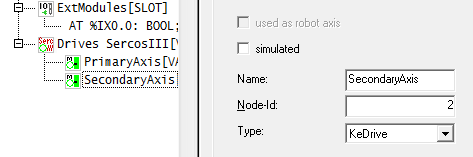
\includegraphics[width=9 cm]{images/DriveConfiguration} 
    \caption{Basiskonfiguration des sekundären Motors}
  \end{minipage}
\end{figure}

\subsubsection{Der Motion Task}
Der "'Motion Task"' dient dazu die Winkelstellungen der Motoren zu aktualisieren, hierzu wird in vom System vorgegebenen Abständen das Programm \textit{McMain} aufgerufen. Das genannte Hauptprogramm überprüft zuerst ob alle zur initialisierung notwendigen Schritte getätigt wurden und geht dann dazu über zuerst die aktuellen Winkelstellungen auszulesen, neue Soll-Werte zu setzen und diese Schließlich an die Motorsteuerungen weiterzugeben. 

Das setzen der neuen Winkelstellungen, sowie alle anderen Operation die eine Veränderung des Zustands der Motoren mit sich bringen passiert im Programm \textit{UserUpdate} welches zwischen dem Lesen der Ist-Werte und dem schreiben der Soll-Werte aufgerufen wird.

\subsubsection{Das UserUpdate Programm}
Das \textit{UserUpdate} Programm dient wie bereits erwähnt zum verändern des Zustands der Motoren. Das Programm ähnelt im Aufbau dem \textit{NetworkManager} Programm sehr stark da es ebenfalls über eine \textit{Switch} Kontrollstruktur gesteuert wird. Für eine genauere Beschreibung dieser Art von Programmaufbau siehe Unterkapitel "'Aufbau"' im Kapitel "'Die Netzwerkkommunikation"'.

Im initialen Status (\textit{state} = 0) beginnt das \textit{UserUpdate} Programm zuerst damit die einzelnen Motoren zu "'resetten"', dies ist notwendig um etwaige Fehler oder unbrauchbare Einstellungen aus der Motorsteuerung zu löschen. Die Operationen an den Motoren werden jeweils über vom System bereitgestellte Funktionsblöcke durchgeführt, welche zur richtigen Zeit mit den entsprechenden Parametern aufgerufen werden. Meist verfügt ein für eine Operation nötiger Funktionsblock über einen \textit{Execute} Parameter, welcher eine positive Flanke aufweisen muss damit die Operation durchgeführt wird. Aus diesem Grund ist es nötig die Funktionsblöcke zweimal aufzurufen, am Beispiel der "'reset"' Operation sieht dies folgendermaßen aus:
\begin{lstlisting}[language = codesysls, captionpos=b, caption={Resetten einer Motors}]
fb_reset_primaryAxis(Axis := SecondaryAxis, Execute := FALSE);
fb_reset_primaryAxis(Axis := SecondaryAxis, Execute := TRUE);
\end{lstlisting}

Nachdem dieser Schritt ausgeführt wurde, wird \textit{state} auf 1 gesetzt. 

Befindet sich das Programm im Status 1, so wird zuerst überprüft ob das "'resetten"' der Motorsteuerungen abgeschlossen ist. Ist dies der Fall, so wird der Funktionsblock für das "'resetten"' erneut aufgerufen um dem \textit{Execute} Parameter den Wert \textit{FALSE} zuzuweisen und damit den Motor für weitere Operationen freizugeben.
Nach Abschluss dieser Operation wird die \textit{state} Variable des Programms auf 10 gesetzt um beim nächsten Programmaufruf die Motoren einzuschalten.

Der nächste Schritt im Programm ist das Einschalten der Motoren, dies geschieht wieder über Aufruf des entsprechenden Funktionsblocks (\textit{MC\_Power}, muss zuvor instanziert worden sein). War das Einschalten der Motoren erfolgreich, so wechselt das Programm in den Status 12.

Im Status 12 überprüft das \textit{UserUpdate} Programm ob ein "'Homing"' also eine Suche nach der Ausgangsposition durchgeführt werden muss. Diese Überprüfung findet mithilfe der globalen Variable \textit{robot\_homing} stattd die gegebenenfalls durch das \textit{NetworkManager} Programm auf den Wert \textit{true} gesetzt wurde.
Da im Rahmen dieses Projektes keine Mechanik erstellt wurde, war das eigentliche "'Homing"' nicht implementierbar und es wird hier Fall lediglich die globale Variable \textit{robot\_homing} auf \textit{false} gesetzt. Zusätzlich wird die globale Variable \textit{robot\_ready} auf \textit{true} gesetzt um dem \textit{NetworkManager} Programm zu signalisieren dass der Roboter bereit ist Befehle zu empfangen. Das \textit{NetworkManager} Programm gibt diese Information an den Computer weiter. Am Ende wird die \textit{state} Variable auf 20 gesetzt.

Hat die \textit{state} Variable den Wert 20, so wartet der "'Motion Task"' auf neue Interpolationspunkte in Form von Winkelstellungen. Werden neue Interpolationspunkte durch das \textit{NetworkManager} Programm eingelesen, so werden sie in globale Array gespeichert, siehe Unterkapitel "'Ablauf des Datenempfanngs"' im Kapitel "'Netzwerkkommunikation"'. Wenn alle Werte fertig eingelesen wurden, wird die globale Variable \textit{stepsAvailable} auf die Länge des Array gesetzt. Hat die genannte Variable nun einen Wert der höher als 0 ist, so wird der erste Winkel aus dem Array an die Motorsteuerung als relativ zu verfahrender Winkel weitergegeben. Die Variable \textit{stepsAvailable} wird nun um 1 verringert und die Variable \textit{curStepIndex} wird um 1 erhöht. Die genannte \textit{curStepIndex} Variable ist zu Anfang 0 und dient dazu zu speichern welcher Schritt aus dem Array beim nächsten Aufruf des \textit{UserUpdate} Programms gefahren werden soll.
\begin{lstlisting}[language = codesysls, captionpos=b, caption={Übergabe der Winkel an die Motoren}]
20: (* Start relative Movement *)

		IF(stepsAvailable > 0)THEN

		fb_moveRelative_primaryAxis(Axis := PrimaryAxis, Execute := FALSE);
		fb_moveRelative_primaryAxis(Axis := PrimaryAxis, Execute := TRUE, Distance := primarySteps[currentStepIndex], Velocity := 300, Acceleration := 10000, Deceleration := 10000);

		fb_moveRelative_secondaryAxis(Axis := SecondaryAxis, Execute := FALSE);
		fb_moveRelative_secondaryAxis(Axis := SecondaryAxis, Execute := TRUE, Distance := primarySteps[currentStepIndex], Velocity := 300, Acceleration := 10000, Deceleration := 10000);

		currentStepIndex := currentStepIndex +1;
		stepsAvailable := stepsAvailable -1;
		END_IF;
\end{lstlisting}

Wurden alle Schritte gefahren, so wird die Variable \textit{robot\_ready} auf true gesetzt. 

Wird im Status 20 durch Kontrolle der \textit{robot\_shutdown} Variable erkannt dass der Roboter heruntergefahren werden soll, so wird \textit{state} auf 100 gesetzt. Damit werden beim nächsten Aufruf des Programms die  Motoren abgeschaltet.




